%!TEX program = xelatex
\documentclass[12pt, a4paper, oneside]{ctexart}
\usepackage[utf8]{inputenc}
\usepackage{ctex} %导入中文包
\usepackage{listings}
\usepackage{fontspec}
\usepackage{geometry} %设置页边距的包
\usepackage{listings}
\usepackage{xcolor} 

\usepackage{graphicx}
\usepackage{float}


\title{\fontsize{70}{30}\selectfont  ACM 模板} 
\author{无敌爆哥} 
\date{\today} 

\geometry{left=2.5cm,right=2cm,top=2.54cm,bottom=2.54cm} %设置书籍的页边距
\definecolor{mygray}{rgb}{0.97,0.97,0.97}%定制颜色

\setsansfont{Monaco} 
\setmainfont{Monaco}

%对于lstset排版
\lstset{
tabsize=4,
	breaklines, 					% 自动将长的代码行换行排版
	backgroundcolor = \color{white},     			 % 背景色:淡黄
	numbers=left, 									% 行号在左侧显示
	numberstyle= \small, 								% 行号字体
	keywordstyle= \color{ red!70},						 % 关键字颜色
	commentstyle= \color{red!50!green!50!blue!50}, 		% 注释颜色
	rulesepcolor= \color{ red!20!green!20!blue!20} ,
	frame=single,                               % 设置代码框形式
	escapeinside=``,									 % 英文分号中可写入中文
	xleftmargin=2em,xrightmargin=2em, aboveskip=1em,
	framexleftmargin=2em
} 


\begin{document} 

\maketitle
\thispagestyle{empty}
\centering

\includegraphics[scale=0.55]{pic.jpg}

\newpage
\tableofcontents 
\thispagestyle{empty}
\lstset{language=C++}

\newpage 
\section{数学} 
\subsection{康托展开} 
可以O(nlogn)复杂度求一个排列对于排列中的排名
\begin{lstlisting}
const int N=1e6+10,mod=998244353;
long long fac[N];
int tr[N];
int n;
int a[N];
int lowbit(int x)
{
	return x&-x;
 } 
void add(int x)
{
	for(int i=x;i<=n;i+=lowbit(i)) tr[i]+=1;
}
int qr(int x)
{
	int res=0;
	for(int i=x;i;i-=lowbit(i)) res+=tr[i];
	return res;
}
long long cantor(){
	fac[0]=1;
	for(int i=1;i<=n;i++) {
		fac[i]=fac[i-1]*i%mod;
	}
	long long ans=0;
	for(int i=1;i<=n;i++){
		ans=(ans+(a[i]-1-qr(a[i]))*fac[n-i]%mod)%mod;
		add(a[i]);
	}
	return (ans+1)%mod;
}
\end{lstlisting}

\newpage 
\subsection{逆康托展开} 
已经知道排名得到原排列,逆向推出原序列
\begin{lstlisting}
vector<int> incantor(int x,int n) {
    x--;// 得到以0开始的排名
    vector<int> res(n);// 保存数列答案
    int cnt;
    bool st[10];// 标记数组
    memset(st,0,sizeof st);
    for(int i = 0;i < n; ++i) {
        cnt = x/fact[n - i - 1];// 比a[i]小且没有出现过的数的个数
        x %= fact[n - i - 1];// 更新 x
        for(int j = 1;j <= n; ++j) {// 找到a[i],从1开始向后找
            if(st[j]) continue;// 如果被标记过,就跳过
            if(!cnt) {// 如果cnt == 0说明当前数是a[i]
                st[j] = 1;//标记
                res[i] = j;// 第i位是j
                break;
            }
            cnt --;// 如果当前不是0,就继续往后找
        }
    }
    return res;// 返回答案
}
\end{lstlisting}

\newpage 
\subsection{线性筛求因子数量} 
\begin{lstlisting}
int fac[N],q[N],top;
bool vis[N];
int cnt[N];
void init(int n=1e6)
{
	vis[1]=true;
	fac[1]=1;
	for(int i=2;i<=n;i++)
	{
		if(vis[i]==false)
		{
			q[top++]=i;
			fac[i]=2;
			cnt[i]=1;
		}
		for(int j=0;1ll*q[j]*i<=n;j++)
		{
			int nu=i*q[j];
			vis[nu]=true;
			if(i%q[j]==0)
			{
				fac[nu]=fac[i]/(cnt[i]+1)*(cnt[i]+2);
				cnt[nu]=cnt[i]+1;
				break;
			}
			fac[nu]=fac[i]*fac[q[j]];
			cnt[nu]=1;
		}
	}
}
\end{lstlisting}

\newpage 
\subsection{二进制GCD} 
快!
\begin{lstlisting}
int gcd(int a, int b) {
    int az = __builtin_ctz(a);
    int bz = __builtin_ctz(b);
    int z = min(az, bz);
    b >>= bz;
    while (a) {
        a >>= az;
        int diff = a - b;
        az = __builtin_ctz(diff);
        b = min(a, b), a = abs(diff);
    }
    return b << z;
}
\end{lstlisting}

\newpage 
\subsection{快速gcd} 
预处理值域,常数访问gcd (T取${\sqrt{max}}$)
\begin{lstlisting}
const int M=1e6+10,T=1e3+10;//值域 
bool vis[M];
int q[M],cnt;
int fac[M][3];
int gc[T][T];
int gcd(int a,int b)
{
	return b?gcd(b,a%b):a;
}
void init(int n=M-10)
{
	vis[1]=true;
	vis[0]=true;
	fac[1][0]=fac[1][1]=fac[1][2]=1;
	for(int i=2;i<=n;i++)
	{
		if(!vis[i])
		{
			q[cnt++]=i;
			fac[i][0]=fac[i][1]=1;
			fac[i][2]=i;
		}
		for(int j=0;1ll*q[j]*i<=n;j++)
		{
			int nu=q[j]*i;
			vis[nu]=true;
			fac[nu][0]=fac[i][0]*q[j];
			fac[nu][1]=fac[i][1];
			fac[nu][2]=fac[i][2];
			if(fac[nu][0]>fac[nu][1]) swap(fac[nu][0],fac[nu][1]);
			if(fac[nu][1]>fac[nu][2]) swap(fac[nu][1],fac[nu][2]);
			if(i%q[j]==0) break;
		}
	}
	for(int i=0;i<=T-10;i++)
	{
		for(int j=0;j<=T-10;j++)
		{
			if(!i&&!j) continue;
			gc[i][j]=gcd(i,j);
		}
	}
}
int qgcd(int x,int y)
{
	int res=1;
	for(int i=0,t=1;i<3;i++)
	{
		if(fac[x][i]>T-10)
		{
			if(y%fac[x][i]) t=1;
			else t=fac[x][i];
		}
		else t=gc[fac[x][i]][y%fac[x][i]];
		res=res*t;y/=t;
	}
	return res;
}
\end{lstlisting}

\newpage 
\subsection{求矩阵行列式值} 
原理是通过高斯消元将行列式下三角清0,那么答案就是主对角线的累乘,这里由于模值不一定是质数,不能保障每一个元素都在P取模情况下有逆元,所以采用了特别妙的方法,通过主元行与其他行进来辗转相除来进行清0过程。原理是行列式中一行减去另外一行的乘积,行列式答案不变。
\begin{lstlisting}
int mod=998244353;
const int N=610;
long long mp[N][N];
int n;
long long gauss()//求矩阵行列式的值
{
	long long res=1;
	for(int i=0;i<n;i++)
	{
		for(int j=i+1;j<n;j++)
		{
			while(mp[i][i])
			{
				long long div=mp[j][i]/mp[i][i];
				for(int k=i;k<n&&div;k++) {
					mp[j][k]=((mp[j][k]-div*mp[i][k])%mod+mod)%mod;
				}
				for(int k=i;k<n;k++) swap(mp[i][k],mp[j][k]);res=-res;
			}
			for(int k=i;k<n;k++) swap(mp[i][k],mp[j][k]);res=-res;
		}
	}
	res=(res+mod)%mod;
	for(int i=0;i<n;i++) res=res*mp[i][i]%mod;
	return res;
}
\end{lstlisting}

\newpage 
\subsection{线性基} 
\begin{lstlisting}
struct Vec{
    vector<long long>d,g;
    int n;
    int le;
    Vec(){};
    Vec(int _n){n=_n;d.resize(n+1);g.resize(n+1);}
    bool insert(long long x){
        for(int i=n;i>=0;i--){
            if((x>>i)&1){
                if(d[i]==0){
                    d[i]=x;
                    return true;
                }else{
                    x^=d[i];
                }
            }
        }
        return false;
    }
    void re(){
        for(int i=0;i<=n;i++){
            for(int j=i-1;j>=0;j--){
                if((d[i]>>j)&1){
                    d[i]^=d[j];
                }
            }
        }
        le=0;
        for(int i=0;i<=n;i++){
            if(d[i]){
                g[le++]=d[i];
            }
        }
    }
    long long qrk(long long x){
        if(x>(1ll<<le)) return -1;   
        x--;
        long long res=0;
        for(int i=0;i<le;i++){
            if((x>>i)&1){
                res^=g[i];
            }
        }
        return res;
    }
};
\end{lstlisting}

\newpage 
\subsection{拓展中国剩余定理(EXCRT)} 
CRT 求的问题是有一个数余上不同的模值M之后,求余数R值\par
通过公式分析可以推出 最终的模值为 M=LCM(m1,m2,m3..) ,R=LCM*k+q.m1+r1\par
有时候如果可以用中国剩余定理搞的题目,需要质数分别当模数,如果wa了试一下不用5什么的
\begin{lstlisting}
long long gcd(long long a,long long b)
{
	return b?gcd(b,a%b):a;
}
long long exgcd(long long a,long long b,long long &x,long long &y)
{
	if(b==0)
	{
		x=1;
		y=0;
		return a;
	}
	long long x1,y1,d;
	d=exgcd(b,a%b,x1,y1);
	x=y1;
	y=x1-a/b*y1;
	return d;
}
long long lcm(long long a,long long b)
{
	return a/gcd(a,b)*b;
}
long long m[20],r[20];
int tp;
long long CRT()
{
	for(int i=1;i<tp;i++)
	{
		long long d,x,y;
		d=exgcd(m[i-1],m[i],x,y);
        if((r[i]-r[i-1])%d) return -1;
		x=x*(r[i]-r[i-1])/d;
		x=(x%(m[i]/d)+m[i]/d)%(m[i]/d);
		r[i]=m[i-1]*x+r[i-1];
		m[i]=lcm(m[i-1],m[i]);
		r[i]=(r[i]%m[i]+m[i])%m[i];
	}
	return r[tp-1]%m[tp-1];
}
\end{lstlisting}
解 at[i]*x\%m[i]=r[i]//带有系数的excrt
\begin{lstlisting}
long long CRT()
{
	tp=n;
	long long ans=0,M=1,A,B,C,x,y;
	for(int i=1;i<=tp;i++)
	{
		A=(__int128)at[i]*M%m[i];
		B=m[i];
		C=(r[i]-at[i]*ans%m[i]+m[i])%m[i];
		long long d=exgcd(A,B,x,y);
		if(C%d) return -1;
		x=(x%B+B)%B;
		ans+=(__int128)(C/d)*x%(B/d)*M%(M*=B/d);
		ans%=M;
	}
	return ans;
}
\end{lstlisting}

\newpage 
\subsection{BSGS} 
${a^x=b(mod p)}$
\begin{lstlisting}
long long gcd(long long a,long long b)
{
	return b?gcd(b,a%b):a;
}
long long BSGS(long long a,long long b,long long p)
{
	a%=p,b%=p;
	if(b==1||p==1){
		return 0;
	}
	int k=0;
	long long A=1;
	while(1)
	{
		long long d=gcd(a,p);
		if(b%d!=0) {
			return -1;
		}
		if(d==1) break;
		k++;b/=d;p/=d;A=A*(a/d)%p;b%=p;
		if(A==b) {
			return k;
		}
	}
	long long m=ceil(sqrt(p));
	map<long long,int>mp;
	long long t=b;
	for(int i=0;i<m;i++)
	{
		mp[t]=i;
		t=t*a%p;
	}
	t=1;
	for(int i=1;i<=m;i++)
	{
		t=t*a%p;
	}
	long long tt=A;
	for(int i=1;i<=m;i++)
	{
		tt=tt*t%p;
		if(mp.count(tt)&&i*m-mp[tt]>=0)
		{
			return i*m-mp[tt]+k;
		}
		
	}
	return -1;
}
\end{lstlisting}

\newpage 
\subsection{卢卡斯求组合数} 
满足mod为质数
\begin{lstlisting}
long long lucas(long long n,long long m)
{
	if(m==0) return 1;
	return lucas(n/mod,m/mod)*C(n%mod,m%mod)%mod;
}
\end{lstlisting}

\subsection{错排} 
n个不相同盒子和n个不相同球,对应球不能放到下标相同盒子中
\begin{lstlisting}
f[0]=1;
f[1]=0;
f[2]=1;
f[i]=(f[i-1]+f[i-2])*(i-1);
\end{lstlisting}

\newpage 
\subsection{高精度} 
\begin{lstlisting}
struct BigInt{
    int w=6;
    int tw=1e6;
    vector<int>v;
    int len=0;
    BigInt(){len=0;}
    BigInt(int _len){len=_len;v.resize(len);}
    BigInt operator +(const BigInt &w)const{
        BigInt res;
        res.v=v;
        res.len=len;
        long long tp=0;
        for(int i=0;i<(int)v.size();i++){
            if(i<(int)w.v.size()){
                tp+=w.v[i];
            }
            tp+=v[i];
            res.v[i]=(tp%tw);
            tp/=tw;
        }
        while(tp) res.v.push_back(tp%tw),tp/=tw,res.len++;
        return res;
    }
    BigInt operator +(const int &x)const{
        int tp=x;
        BigInt res;
        res.v=v;
        res.len=len;
        for(int i=0;i<(int)v.size();i++){
            tp+=v[i];
            res.v[i]=(tp%tw);
            tp/=tw;
            if(tp==0) break;
        }
        while(tp) res.v.push_back(tp%tw),tp/=tw,res.len++;
        return res;
    }
    //sub只有a>=b
    BigInt operator -(const BigInt &w)const{
        BigInt res;
        res.v=v;
        res.len=len;
        for(int i=0;i<len;i++){
            if(i<(int)w.len){
                res.v[i]-=w.v[i];
            }
            if(res.v[i]<0) res.v[i]+=tw,res.v[i+1]--;
        }
        while(res.len>1&&res.v.back()==0){
            res.v.pop_back();
            res.len--;
        }
        return res;
    }
    BigInt operator - (const int b)const{
        BigInt res;
        res.v=v;
        res.len=len;
        res.v[0]-=b;
        for(int i=0;i<(int)v.size();i++){
            while(res.v[i]<0) res.v[i]+=tw,res.v[i]--;
        }
        while(res.len>1&&res.v.back()==0){
            res.v.pop_back();res.len--;
        }
        return res;
    }
    BigInt operator *(const BigInt & w)const{
        BigInt res(len+w.len+2);
        for(int i=0;i<len;i++){
            for(int j=0;j<w.len;j++){
                long long tp=1ll*v[i]*w.v[j];
                res.v[i+j+1]+=tp/tw;
                res.v[i+j]+=tp%tw;
                res.v[i+j+1]+=res.v[i+j]/tw;
                res.v[i+j]%=tw;
            }
        }
        while(res.len>1&&res.v.back()==0){
            res.v.pop_back();res.len--;
        }
        return res;
    }
    BigInt operator *(const int  w)const{
        BigInt res;
        res.v=v;
        res.len=len;
        long long tp=0;
        for(int i=0;i<len;i++){
            tp+=1ll*w*res.v[i];
            res.v[i]=tp%tw;
            tp/=tw;
        }
        while(tp){
            res.v.push_back(tp%tw);res.len++;
            tp/=tw;
        }
        return res;
    }
    BigInt operator /(const int w)const{
        BigInt res;
        res.v=v;
        res.len=len;
        long long tp=0;
        for(int i=len-1;i>=0;i--){
            tp=tp*tw+v[i];
            res.v[i]=tp/w;
            tp%=w;
        }
        while(res.len>1&&res.v.back()==0){
            res.v.pop_back();res.len--;
        }
        return res;
    }
    int operator %(const int w)const{
        long long res=0;
        for(int i=len-1;i>=0;i--){
            res=res*tw+v[i];
            res%=w;
        }    
        return res;
    }
    void read(string &a){
        for(int i=(int)a.size();i-1>=0;i-=w){
            int res=0;
            for(int j=max(0,i-w);j<=i-1;j++){
                res=res*10+(a[j]-'0');
            }
            v.push_back(res);len++;
        }
    }
    /*
    1 a>b
    -1 a<b
    0 a=b
    */
    int equal(const BigInt &w){
        if(len>w.len) return 1;
        else if(len<w.len) return -1;
        for(int i=len-1;i>=0;i--){
            if(v[i]>w.v[i]) return 1;
            else if(v[i]<w.v[i]) return -1;
        }
        return 0;
    }
    void pr(){
        if(len==1){
            cout<<v[0];
        }
        else{
            int f=0;
            for(int i=len-1;i>=0;i--){
                int x=v[i];
                int tww=tw;
                for(int j=0;j<w;j++){
                    tww/=10;
                    int y=x/tww;
                    if(y) f=1;
                    if(f) cout<<y;
                    x%=tww;
                }
            }
        }
        cout<<'\n';
    }
};
\end{lstlisting}

\newpage 
\subsection{高精度GCD} 
\begin{lstlisting}
BigInt gcd(BigInt a,BigInt b){
    int tp=0;
    while(1){
        int t=a.equal(b);
        if(t==-1) swap(a,b);
        if(t==0||b.len==1&&b.v[0]==0) break;
        if(!(a.v[0]&1)&&!(b.v[0]&1)){
            tp++;
            a=a/2;
            b=b/2;
        }
        else if(!(a.v[0]&1)){
            a=a/2;
        }
        else if(!(b.v[0]&1)){
            b=b/2;
        }else{
            a=a-b;
        }
    }
    while(tp--){
        a=a*2;
    }
    return a;
}
\end{lstlisting}

\newpage 
\subsection{拉格朗日插值} 
${f(x)=\sum_{i=1}^ny_i\prod_{j=1}^n\frac{x-x_j}{x_i-x_j}(x_i \neq x_j)}$
\begin{lstlisting}
const int N=2e5+10,mod=998244353;
long long ksm(long long a,long long b){
    long long res=1;
    a%=mod;
    while(b){
        if(b&1) res=res*a%mod;
        a=a*a%mod;
        b>>=1;
    }
    return res;
}
struct pp{
    long long x,y;
}p[N];
int n;
long long lagrange(long long k){
    long long ans=0;
    for(int i=1;i<=n;i++){
        long long res=1;
        long long res1=1;
        for(int j=1;j<=n;j++){
            if(i==j) continue;
            res=res*(p[i].x-p[j].x+mod)%mod;
            res1=res1*(k-p[j].x+mod)%mod;
        }
        ans=(ans+p[i].y*res1%mod*ksm(res,mod-2)%mod)%mod;
    }
    return ans;
}
\end{lstlisting}

\newpage 
\subsection{FFT(快速傅里叶变换)} 
系数表示法—>点值表示法—>系数表示法\par
采用单位根,运用负数表达,系数需要小数表达可以选择fft
\begin{lstlisting}
const int N=3e6+10;
int r[N];
int n,m;
const double PI=acos(-1);
struct complex_{
	double a,b;
	complex_(){a=0;b=0;}
	complex_(double _a,double _b){a=_a;b=_b;}
	complex_ operator +(const complex_ &w)const{
		return complex_(a+w.a,b+w.b);
	}
	complex_ operator -(const complex_ &w)const{
		return complex_(a-w.a,b-w.b);
	}
	complex_ operator *(const complex_ &w)const{
		return complex_(a*w.a-b*w.b,a*w.b+b*w.a);
	}
};
struct FFT{
	vector<complex_>v;
	int len;
	FFT(){}
	FFT(int _len){v.resize(_len);len=_len;}
	void init(int _len){
		v.resize(_len);
		len=_len;
	}
	void fft(int type){
		for(int i=0;i<len;i++){
			if(i<r[i]) swap(v[i],v[r[i]]);
		}
		for(int mid=1;mid<len;mid<<=1){
			complex_ wn(cos(PI/mid),type*sin(PI/mid));
			for(int R=mid<<1,j=0;j<len;j+=R){
				complex_ w(1,0);
				for(int k=0;k<mid;k++,w=w*wn){
					complex_ x=v[j+k],y=w*v[j+k+mid];
					v[j+k]=x+y;
					v[j+k+mid]=x-y;
				}
			}
		}
	}
 	void mul(const FFT &w){
 		for(int i=0;i<len;i++){
 			v[i]=v[i]*w.v[i];
 		}
 	}
};
int limit,top;
void init(){
	limit=1;top=0;
	while(limit<=n+m) limit<<=1,top++;
	for(int i=0;i<limit;i++){
		r[i]=(r[i>>1]>>1)|((i&1)<<(top-1));
	}
}
\end{lstlisting}

\newpage 
\subsection{原根} 
若${gcd(a,m)==1}$同时${a^x\equiv1(mod m)}$的最小阶为$\phi(m)$则表示a是m的原根\par
求解通常是暴力算,已经被证明原根渐近$m^\frac{1}{4}$ 所以时间还是比较可观\par
且只有 2,4,${p^a}$ ,${2p^a}$(p为奇质数)才有原根
\begin{lstlisting}
int n,d;
    cin>>n>>d;
    if(!vvis[n]){ //通过线性筛预处理出 2 4 p^a 2p^a
        cout<<"0\n";
        cout<<'\n';
    }else{
        int t=getol(n);//获得欧拉函数
        vector<int>pr=getpr(t);//获得质因子
        int fas=0;
        for(int g=1;;g++){
            int f=0;
            if(__gcd(g,n)!=1) continue;
            //因为阶是n的欧拉函数,所以因子都不能满足
            for(int v:pr){ 
                if(ksm(g,t/v,n)==1){
                    f=1;break;
                }
            }
            if(f==0){
                fas=g;break;//最小原根
            }
        }
        vector<int>ans;
        int num=fas;
        //所有原根
        for(int i=1;i<=t;i++){
            if(__gcd(i,t)==1){
                ans.push_back(num);
            }
            num=num*fas%n;
        }
    }
\end{lstlisting}

\newpage 
\subsection{NTT(快速数论变换)} 
采用原根来表达,都为整数运算,可以相对fft减少精度的影响。
\begin{lstlisting}
/*
65537
998244353
1004535809
4179340454199820289
因为ntt受限制模数需要p=r*2^l+1 (其中l需要比给定运算的多项式的log(len)要大)
所有以上是常见的 且g=3 如果遇到一个其余模数,可以先预处理看是否符合ntt要求在选择ntt求解
*/
\end{lstlisting}
\begin{lstlisting}
const int N=3e6+10;
int r[N];
int limit,L;
void init(int n){
    for(int i=0;i<n;i++){
        r[i]=(r[i>>1]>>1)|((i&1)<<(L-1));
    }
}
struct NTT{
    int len;
    int g=3,gi=332748118;
    long long mod=998244353;
    vector<long long>v;
    NTT(){g=3;gi=332748118;mod=998244353;}
    NTT(int _len){len=_len;v.resize(len);g=3;gi=332748118;mod=998244353;}
    void init(int _len){len=_len;v.resize(len);g=3;gi=332748118;mod=998244353;}
    void ntt(int type){
        for(int i=0;i<len;i++){
            if(i<r[i]) swap(v[i],v[r[i]]);
        }
        for(int mid=1;mid<len;mid<<=1){
            long long wn=ksm(type==1?g:gi,(mod-1)/(mid<<1),mod);
            for(int j=0,R=mid<<1;j<limit;j+=R){
                long long w=1;
                for(int k=0;k<mid;k++,w=(w*wn)%mod){
                    long long x=v[j+k],y=v[j+mid+k]*w%mod;
                    v[j+k]=(x+y)%mod;
                    v[j+k+mid]=(x-y+mod)%mod;
                }
            }
        }
    }
    void mul(const NTT &w){
        for(int i=0;i<len;i++){
            v[i]=(v[i]*w.v[i])%mod;
        }
    }
};
\end{lstlisting}

\newpage 
\subsection{多项式求逆(ntt)} 
\begin{lstlisting}
#include<bits/stdc++.h>
using namespace std;
int read() {
	int q=0;char ch=' ';
	while(ch<'0'||ch>'9') ch=getchar();
	while(ch>='0'&&ch<='9') q=q*10+ch-'0',ch=getchar();
	return q;
}
const int mod=998244353,G=3,N=2100000;

long long ksm(long long a,long long b)
{
	long long res=1;
	a%=mod;
	while(b)
	{
		if(b&1) res=1ll*res*a%mod;
		a=1ll*a*a%mod;
		b>>=1;
	}
	return res;
} 
long long a[N],b[N],c[N];
int r[N];
void NTT1(long long *a,int n,int x) {
	for(int i=0;i<n;++i) if(i<r[i]) swap(a[i],a[r[i]]);
	for(int i=1;i<n;i<<=1) {
		int gn=ksm(G,(mod-1)/(i<<1));
		for(int j=0;j<n;j+=(i<<1)) {
			int t1,t2,g=1;
			for(int k=0;k<i;++k,g=1LL*g*gn%mod) {
				t1=a[j+k],t2=1LL*g*a[j+k+i]%mod;
				a[j+k]=(t1+t2)%mod,a[j+k+i]=(t1-t2+mod)%mod;
			}
		}
	}
	if(x==1) return;
	long long ny=ksm(n,mod-2); reverse(a+1,a+n);
	for(int i=0;i<n;++i) a[i]=1LL*a[i]*ny%mod;
}
void work(int n,long long *a,long long *b) {
	if(n==1) {b[0]=ksm(a[0],mod-2);return;}
	work((n+1)>>1,a,b);
	int l=0,limit=1;
	while(limit<2*n) limit<<=1,++l;
	for(int i=1;i<limit;++i) r[i]=(r[i>>1]>>1)|((i&1)<<(l-1));
	for(int i=0;i<n;++i) c[i]=a[i];
	for(int i=n;i<limit;++i) c[i]=0;
	NTT1(c,limit,1);
	NTT1(b,limit,1);
	for(int i=0;i<limit;++i)
		b[i]=1LL*(2-1LL*c[i]*b[i]%mod+mod)%mod*b[i]%mod;
	NTT1(b,limit,-1);
	for(int i=n;i<limit;++i) b[i]=0;
}
int main()
{
	int n;
	n=read();
	for(int i=0;i<n;++i) a[i]=read();
	work(n,a,b);
	for(int i=0;i<n;++i) printf("%lld ",b[i]);
	return 0;
}
\end{lstlisting}

\newpage 
\subsection{区间维护等差数列} 
当有修改操作等需要给某一段区间加上等差数列,可以通过如下操作来进行维护,最后多用于求某单点值
\begin{lstlisting}
#include<bits/stdc++.h>
using namespace std;
/*
这是无离散化版本
离散化只需要将有下标的地方改成对应 id[下标]即可 
*/
const int N=1e5+10;
int n,q;
int a[N];
struct pp
{
	long long a,d;
}tr[N<<2];

void build(int k,int l,int r)
{
	tr[k].a=tr[k].d=0;
	if(l==r)
	{
		tr[k].a=a[l];
		return;
	}
	int mi=(l+r)>>1;
	build(k<<1,l,mi);
	build(k<<1|1,mi+1,r);
}

void down(int k,int l,int r)
{
	int mi=(l+r)>>1;
	tr[k<<1].d+=tr[k].d;
	tr[k<<1|1].d+=tr[k].d;
	tr[k<<1].a+=tr[k].a;
	tr[k<<1|1].a+=tr[k].a+(mi+1-l)*tr[k].d;
	tr[k].a=tr[k].d=0;
}

void mif(int k,int l,int r,int x,int y,int tp,long long a,long long d)
{
	if(l==x&&r==y)
	{
		tr[k].d+=d;
		tr[k].a+=a+(l-tp)*d;
		return;
	}
	int mi=(l+r)>>1;
	down(k,l,r);
	if(y<=mi) mif(k<<1,l,mi,x,y,tp,a,d);
	else if(mi<x) mif(k<<1|1,mi+1,r,x,y,tp,a,d);
	else mif(k<<1,l,mi,x,mi,tp,a,d),mif(k<<1|1,mi+1,r,mi+1,y,tp,a,d);
}

long long qr(int k,int l,int r,int x)
{
	if(l==x&&r==x)
	{
		return tr[k].a;
	}
	int mi=(l+r)>>1;
	down(k,l,r);
	if(x<=mi) return qr(k<<1,l,mi,x);
	else return qr(k<<1|1,mi+1,r,x);
}

int main()
{
	ios::sync_with_stdio(false);cin.tie(0);cout.tie(0);
	cin>>n>>q;
	for(int i=1;i<=n;i++)
	{
		cin>>a[i];
	}
	build(1,1,n);
	while(q--)
	{
		int op;
		cin>>op;
		if(op==1)
		{
			int l,r;
			long long a,d;
			cin>>l>>r>>a>>d;
			mif(1,1,n,l,r,l,a,d);
		}
		else{
			int x;
			cin>>x;
			cout<<qr(1,1,n,x)<<'\n';
		}
	}
	return 0;
}
\end{lstlisting}

\newpage
\subsection{随机化}
\subsubsection{随机数据生成器} 
\begin{lstlisting}
mt19937 rng(chrono::steady_clock::now().time_since_epoch().count());   //uint
mt19937_64 rng(chrono::steady_clock::now().time_since_epoch().count());//ull  大概率生成不相同数据
int getRand(int l,int r){
    uniform_int_distribution < int > uid(l,r);
    return uid(rng);
}
\end{lstlisting}
\subsubsection{随机排列数组} 
\begin{lstlisting}
random_shuffle(a,a+n);
\end{lstlisting}

\newpage 
\subsection{二项式反演} 
$g_n$表示至多有n个/种方案数量,$f_n$恰好n个/种方案数量\\
\centering
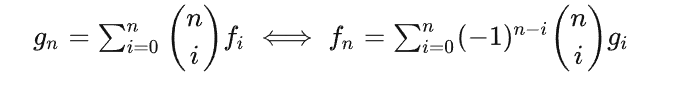
\includegraphics[scale=0.7]{a2.png}
$g_k$表示至少有n个/种方案数量,$f_k$恰好n个/种方案数量\\
\centering
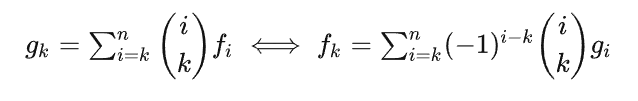
\includegraphics[scale=0.7]{a1.png}
\begin{lstlisting}
\end{lstlisting}

\newpage 
\subsection{Pollard-Rho} 
\begin{lstlisting}
#define LL long long
LL mul(LL a, LL b, LL p) {
    return (a * b - (LL)(a / (long double)p * b + 1e-3) * p + p) % p;
}
LL power(LL a, LL r, LL p) {
    LL res = 1;
    for (; r; a = mul(a, a, p), r >>= 1)
        if (r & 1)
            res = mul(res, a, p);
    return res;
};
bool miller_rabin(LL n) {
    static LL p[9] = {2, 3, 5, 7, 11, 13, 17, 19, 23};
    if (n == 1)
        return false;
    LL d = n - 1, r = 0;
    for (; not(d & 1); d >>= 1)
        r += 1;
    bool res = true;
    for (int i = 0; i < 9 and p[i] < n and res; i += 1) {
        LL x = power(p[i], d, n);
        if (x == 1 or x == n - 1)
            continue;
        for (int j = 1; j < r; j += 1) {
            x = mul(x, x, n);
            if (x == n - 1)
                break;
        }
        if (x != n - 1)
            res = false;
    }
    return res;
};
vector<LL> pollard_rho(LL n) {
    vector<LL> res;
    function<void(LL)> rho = [&](LL n) {
        if (n == 1)
            return;
        if (miller_rabin(n))
            return res.push_back(n), void();
        LL d = n;
        while (d == n) {
            d = 1;
            for (LL k = 1, y = 0, x = 0, s = 1, c = rand() % n; d == 1;
                 k <<= 1, y = x, s = 1) {
                for (int i = 1; i <= k; i += 1) {
                    x = (mul(x, x, n) + c) % n;
                    s = mul(s, abs(x - y), n);
                    if (not(i % 127) or i == k) {
                        d = __gcd(s, n);
                        if (d != 1)
                            break;
                    }
                }
            }
        }
        rho(d);
        rho(n / d);
    };
    rho(n);
    return res;
}
\end{lstlisting}

\newpage 
\subsection{杜教筛} 
能够在 ${O(n^\frac{2}{3})}$的时间负责度里求前n项积性函数的和   \par
${g(1)s(n)}=\sum_{i=1}^n(f*g)(i)-\sum_{i=2}^ng(i)s(\lfloor\frac{n}{i}\rfloor)$ \par
前n项目欧拉函数和莫比乌斯函数和
\begin{lstlisting}
const int N=3e6+10;
int q[N],cnt;
long long u[N],o[N];
bool vis[N];
long long sumol[N],sumu[N];
void init(int n=N-10)
{
	vis[1]=true;
	o[1]=1;
	u[1]=1;
	for(int i=2;i<=n;i++)
	{
		if(vis[i]==false)
		{
			q[cnt++]=i;
			u[i]=-1;
			o[i]=i-1;
		}
		for(int j=0;1ll*q[j]*i<=n;j++)
		{
			int nu=q[j]*i;
			vis[nu]=true;
			if(i%q[j]==0)
			{
				u[nu]=0;
				o[nu]=o[i]*q[j];
				break;
			}
			u[nu]=-u[i];
			o[nu]=o[i]*(q[j]-1);
		}
	}
	for(int i=1;i<=n;i++)
	{
		sumol[i]=sumol[i-1]+o[i];
		sumu[i]=sumu[i-1]+u[i];
	}
}
map<long long,long long>mpo,mpu;
long long get_o(long long n)//前n项欧拉函数的和
{
	if(n<=N-10) return sumol[n];
	if(mpo.count(n)) return mpo[n];
	long long ans=1ll*n*(n+1)/2;
	for(long long int l=2,r;l<=n;l=r+1)
	{
		r=n/(n/l);
		ans-=get_o(n/l)*(r-l+1);
	}
	return mpo[n]=ans;
}

long long get_u(long long n)//前n项莫比乌斯函数的和
{
	if(n<=N-10) return sumu[n];
	if(mpu.count(n)) return mpu[n];
	long long ans=1;
	for(long long int l=2,r;l<=n;l=r+1)
	{
		r=n/(n/l);
		ans-=get_u(n/l)*(r-l+1);
	}
	return mpu[n]=ans;
}
\end{lstlisting}

\newpage 
\subsection{伯特兰-切比雪夫定理} 
若整数n>3,则至少存在一个质数P,符合n<P<2*n-2 ,一个稍弱说法,一个大于1的整数,至少存在一个质数P,符合n<P<2*n


\subsection{基础博弈论} 
\begin{lstlisting}
一. 巴什博奕(Bash Game):

A和B一块报数,每人每次报最少1个,最多报4个,看谁先报到30。这应该是最古老的关于巴什博奕的游戏了吧。

其实如果知道原理,这游戏一点运气成分都没有,只和先手后手有关,比如第一次报数,A报k个数,那么B报5-k个数,那么B报数之后问题就变为,A和B一块报数,看谁先报到25了,进而变为20,15,10,5,当到5的时候,不管A怎么报数,最后一个数肯定是B报的,可以看出,作为后手的B在个游戏中是不会输的。

那么如果我们要报n个数,每次最少报一个,最多报m个,我们可以找到这么一个整数k和r,使n=k*(m+1)+r,代入上面的例子我们就可以知道,如果r=0,那么先手必败;否则,先手必胜。

二. 威佐夫博弈(Wythoff Game):

有两堆各若干的物品,两人轮流从其中一堆取至少一件物品,至多不限,或从两堆中同时取相同件物品,规定最后取完者胜利。

直接说结论了,若两堆物品的初始值为(x,y),且x<y,则另z=y-x;

记w=(int)[((sqrt(5)+1)/2)*z ];

若w=x,则先手必败,否则先手必胜。

三. 尼姆博弈(Nimm Game):

尼姆博弈指的是这样一个博弈游戏:有任意堆物品,每堆物品的个数是任意的,双方轮流从中取物品,每一次只能从一堆物品中取部分或全部物品,最少取一件,取到最后一件物品的人获胜。

结论就是:把每堆物品数全部异或起来,如果得到的值为0,那么先手必败,否则先手必胜。

四. 斐波那契博弈:

有一堆物品,两人轮流取物品,先手最少取一个,至多无上限,但不能把物品取完,之后每次取的物品数不能超过上一次取的物品数的二倍且至少为一件,取走最后一件物品的人获胜。

结论是:先手胜当且仅当n不是斐波那契数(n为物品总数)
\end{lstlisting}

\newpage 
\section{几何}
能不用浮点就不用 
\subsection{几何通用}
\begin{lstlisting}
//#define double long double//wa了就试一下
const double eps=1e-12;
const double pi=acos(-1);
int cmpb(double x)
{
    if(fabs(x)<eps) return 0;
    if(x>0) return 1;
    return -1;
}
struct point{
    double x,y;
    point(){x=0;y=0;}
    point(double _x,double _y){x=_x;y=_y;};
    double operator |(const point &w) const//点乘
    {
        return x*w.x+y*w.y;
    }
    double operator ^(const point &w) const//叉乘
    {
        return x*w.y-y*w.x;
    }
    point operator -(const point &w) const
    {
        point res;
        res.x=x-w.x;res.y=y-w.y;
        return res;
    }
    point operator +(const point &w) const
    {
        point res;
        res.x=x+w.x;res.y=y+w.y;
        return res;
    }
    point operator /(double w) const
	{
    	point res(x/w,y/w);
		return res;	
	}
	point operator *(double w) const
	{
    	point res(x*w,y*w);
		return res;	
	}
    double db(double x)   //平方
    {
        return x*x;
    }
    double dict(point &to)//点距
    {
        return sqrt(db(x-to.x)+db(y-to.y));
    }
    double dz()
    {
    	return sqrt(db(x)+db(y));
	}
	void rotate(double _o) //旋转都是逆时针 
	{
		double _x=x,_y=y;
		x=_x*cos(_o)-_y*sin(_o);
    	y=_x*sin(_o)+_y*cos(_o);
	}
    double arg()//绕正x轴旋转多少度到达
    {
        int xb=cmpb(x),yb=cmpb(y);
        if(xb==0&&yb==0) return 0.0;
        if(yb==0)
        {
            if(xb==1) return 0.0;
            else return pi;
        }
        if(xb==0)
        {
            if(yb==1) return pi/2.0;
            else return 1.5*pi;
        }
        double ta=fabs(atan(y/x));
        if(xb==1&&yb==-1) ta+=1.5*pi;
        else if(xb==-1&&yb==-1) ta+=pi;
        else if(xb==-1&&yb==1) ta+=0.5*pi;
        return ta;
    }
};
struct Line{
    double a,b,c;     //直线一般式
    Line(){a=0;b=0;c=0;}
    Line(double _a,double _b,double _c)
    {
        a=_a;
        b=_b;
        c=_c;
    }
    Line(point &x,point &y)//俩点一线
    {
        a=y.y-x.y;
        b=x.x-y.x;
        c=x.y*y.x-x.x*y.y;
    }
    point cross(Line &x)   //线交点
    {
        point res;
        res.x=(x.c*b-c*x.b)/(a*x.b-x.a*b);
        res.y=(x.c*a-c*x.a)/(b*x.a-x.b*a);
        return res;
    }
     bool check(point &x)//判断点是否在线上
    {
        return cmpb(x.x*a+x.y*b+c)==0;
    }
    Line getL(point &x){//获得得某点到这个条线的垂直线
        double a1,b1,c1;
        if(a==0) {
            a1=1.0;
            b1=0;
            c1=-x.x;
        }
        else if(b==0)
        {
            a1=0;
            b1=1.0;
            c1=-x.y;
        }
        else{
            a1=b;
            b1=-a;
            c1=a*x.y-b*x.x;
        }
        Line re(a1,b1,c1);
        return re;
    }
    bool Px(Line &w)//判断平行
    {
        return cmpb(a*w.b-b*w.a)==0;
    }
    bool Li(Line &w)//判断垂直
    {
        return cmpb(a*w.b+b*w.a)==0;
    }
};
struct Line //起点 终点版 
{
    point s,e;
    Line(){}
    Line(point _s,point _e){s=_s;e=_e;}
    point cross(Line &W) {
        point u=s-W.s,v=e-s,w=W.e-W.s;
        double t=(u^w)/(w^v);
        return s+v*t;
    }
    bool right(Line b,Line c)//判断b,c交点是否在当前线段右边 
    {
        point p=b.cross(c);
        return ((e-s)^(p-s))<0;
    }
    double arg() //极角 (-pi,pi]
    {
        return atan2(e.y-s.y,e.x-s.x); 
    }
};
double cro(point a,point b,point c)
{
	return (b-a)^(c-a);
}

double dot(point a,point b,point c)
{
	return (b-a)|(c-a);
}

struct point3{//三维 
	double x,y,z;
	point3()
	{
		x=0.0;y=0.0;z=0.0;
	}
	point3(double _x,double _y,double _z)
	{
		x=_x;y=_y;z=_z;
	}
	point3 operator -(const point3 w)
	{
		return (point3){x-w.x,y-w.y,z-w.z};
	}
	point3 operator +(const point3 w)
	{
		return (point3){x+w.x,y+w.y,z+w.z};
	}
	point3 operator ^(const point3 w)
	{
		return (point3){(y*w.z-z*w.y),(z*w.x-x*w.z),(x*w.y-y*w.x)};
	}
	double operator |(const point3 w)
	{
		return x*w.x+y*w.y+z*w.z;
	}
	double rand01()
	{
		return (double)rand()/(double)RAND_MAX;
	}
    double randeps()
    {
        return (double)(rand01()-0.5)*eps; 
    }
	void noise()//三维点需要抖动一下避免有一些影响 十分重要!
	{
		x+=randeps();y+=randeps(),z+=randeps();
	}
	double db(double x)
	{
		return x*x;
	}
	double dict(const point3 w)
	{
		return sqrt(db(x-w.x)+db(y-w.y)+db(z-w.z));
	}
	double mod()
	{
		return sqrt(x*x+y*y+z*z);
	}
};
\end{lstlisting}

\newpage 
\subsection{极角序} 
\begin{lstlisting}
//排序cmp
struct argcmp{//极角排序
    int quad(const point&x) //象限排序 根据题目定义
        {
            if(x.y<-eps) return 1;
            else if(x.y>eps) return 3;
            else if(x.x>eps) return 4;
            else if(x.x<-eps) return 5;
            return 2;
        };
    bool operator()(const point &x,const point &y) 
    {
        
        int xb=quad(x);
        int yb=quad(y);
        if(xb!=yb)
        {
            return xb<yb;
        }
        return (x^y)>eps; //右手定则
    }
};
\end{lstlisting}

\newpage 
\subsection{凸包}
\subsubsection{二维凸包} 
\begin{lstlisting}
const int N=4e5+10;
bool cmp(point x,point y)
{
	return (x.x==y.x?x.y<y.y:x.x<y.x);
}
point st[N],p[N];
int top,tp;
double Andrew()
{
    top=0;//多组清空
	sort(p+1,p+tp+1,cmp);
	for(int i=1;i<=tp;i++)
	{
		while(top>1&&((st[top]-st[top-1])^(p[i]-st[top-1]))<=0.0) top--;
		st[++top]=p[i];
	}
	int t=top;
	for(int i=tp-1;i>=1;i--)
	{
		while(top>t&&((st[top]-st[top-1])^(p[i]-st[top-1]))<=0.0) top--;
		st[++top]=p[i];
 	}
 	double ans=0.0;
 	for(int i=1;i<top;i++)
 	{
 		ans=ans+st[i].dict(st[i+1]);
	}
	return ans;
}
\end{lstlisting}

\newpage 
\subsection{三维凸包} 
\subsubsection{暴力}
\begin{lstlisting}
const int N=110;
point3 p[N];
int n;
bool check(int id,int id1,int id2)
{
	double now=0;
	int c1=0,c2=0;
	point3 vr=(p[id1]-p[id])^(p[id2]-p[id]);
	for(int i=1;i<=n;i++)
	{
		if(i==id||i==id1||i==id2) continue;
		now=((p[i]-p[id])|vr);
		if(now>0)
		{
			c1++;
		}
		else if(now<0){
			c2++;
		}
		if(c1&&c2) return false;
		
	}
	return true;
}
void solve()
{
	scanf("%d",&n);
	for(int i=1;i<=n;i++)
	{
		scanf("%Lf%Lf%Lf",&p[i].x,&p[i].y,&p[i].z);
		p[i].noise();
	}
	double ans=0;
	for(int i=1;i<=n;i++)
	{
		for(int j=i+1;j<=n;j++)
		{
			for(int k=j+1;k<=n;k++)
			{
				if(check(i,j,k))
				{
					ans+=((p[j]-p[i])^(p[k]-p[i])).mod()/2.0; //通过向量积的模长一半求得出 
				}
			}
		}
	}
	printf("%Lf",ans);
}
\end{lstlisting}

\newpage 
\subsection{增量法} 
\begin{lstlisting}
const int N=2010;
point3 p[N];
struct face{
	int v[3];
	face(){v[0]=v[1]=v[2]=0;}
	face(int a,int b,int c){v[0]=a;v[1]=b;v[2]=c;}
	point3 normal(){return ((p[v[1]]-p[v[0]])^(p[v[2]]-p[v[0]]));}
	double area(){return normal().mod()/2.0;}
};
int cansee(face A,point3 b) {return ((b-p[A.v[0]])|A.normal())>0;}
face cv[N],h[N];
int n,th,cnt,vis[N][N];
void convex3() {
	cnt=th=0;
	cv[++cnt]=face(1,2,3);
	cv[++cnt]=face(3,2,1);
	for(int i=4;i<=n;++i) {
		for(int j=1,v;j<=cnt;++j) {
			if(!(v=cansee(cv[j],p[i])))h[++th]=cv[j];
			for(int k=0;k<3;++k) 
				vis[cv[j].v[k]][cv[j].v[k>1?0:k+1]]=v;
		}
		for(int j=1;j<=cnt;++j)
			for(int k=0;k<3;++k) {
				int x=cv[j].v[k],y=cv[j].v[k>1?0:k+1];
				if(vis[x][y]&&!vis[y][x])h[++th]=face(x,y,i);
			}
		for(int j=1;j<=th;++j)cv[j]=h[j];
		cnt=th,th=0;
	}
}
double calc(){
	double res=0;
	for(int i=1;i<=cnt;i++)
	{
		res+=cv[i].area();
	}
	return res;
}
double vol6(point3 a,point3 b,point3 c,point3 d) {
	return ((b-a)^(c-a))|(d-a);
} //计算体积的6倍。理解:先算出底的有向面积的2倍,向量的方向变为高,然后点乘就是另一条边在高方向的投影,由体积公式(V=1/3*Sh),这个值就是体积的6倍
double calcV() {//体积 
	double res=0;
	for(int i=1;i<=cnt;++i)
		res+=fabs(vol6(p[1],p[cv[i].v[0]],p[cv[i].v[1]],p[cv[i].v[2]]));
	res/=6.0;
	return res;
}
\end{lstlisting}

\newpage 
\subsection{线段到线段最小距离} 
\begin{lstlisting}
double cro(point a,point b,point c)
{
    return ((b-a)^(c-a));
}

double dot(point p0,point p1,point p2){  //点积 p0为角点
    return (p1-p0)|(p2-p0);
}
  
double getDis(point p0,point p1,point p2){
     if(cmpb(p0.dict(p1))==0) return p0.dict(p2);//p0 p1共同点
     if(cmpb(dot(p0,p1,p2))==-1) return p2.dict(p0);//钝角
     if(cmpb(dot(p1,p0,p2))==-1) return p2.dict(p1);//钝角
     return fabs(cro(p0,p1,p2)/p0.dict(p1));  //点到线的距离
}
  
double minDis(point p1,point p2,point p3,point p4){//线段间最短距离
     return min(min(getDis(p1,p2,p3),getDis(p1,p2,p4)),min(getDis(p3,p4,p1),getDis(p3,p4,p2)));
}
\end{lstlisting}

\newpage 
\subsection{旋转卡壳} 
\subsubsection{凸包直径}
\begin{lstlisting}
double rotating_calingpers()
{
    top--;
 	double ans=0;
    for(int i=0,j=1;i<top;i++)
    {
        while(((st[(i+1)%top]-st[i])^(st[j]-st[i]))<
              ((st[(i+1)%top]-st[i])^(st[(j+1)%top]-st[i]))){
            j=(j+1)%top;
        }
        ans=max(ans,st[i].dict(st[j]));
        ans=max(ans,st[(i+1)%top].dict(st[j]));
    }
    return ans;
}
\end{lstlisting}

\newpage 
\subsubsection{俩个不相交凸包最小距离} 
\begin{lstlisting}
double cro(point a,point b,point c)
{
    return ((b-a)^(c-a));
}

double dot(point p0,point p1,point p2){  //点积 p0为角点
    return (p1-p0)|(p2-p0);
}
  
double getDis(point p0,point p1,point p2){
     if(cmpb(p0.dict(p1))==0) return p0.dict(p2);//p0 p1共同点
     if(cmpb(dot(p0,p1,p2))==-1) return p2.dict(p0);//钝角
     if(cmpb(dot(p1,p0,p2))==-1) return p2.dict(p1);//钝角
     return fabs(cro(p0,p1,p2)/p0.dict(p1));  //点到线的距离
}
  
double minDis(point p1,point p2,point p3,point p4){//线段间最短距离
     return min(min(getDis(p1,p2,p3),getDis(p1,p2,p4)),min(getDis(p3,p4,p1),getDis(p3,p4,p2)));
}

double r_c(int f)
{
    int ymi=1,ymx=1;
    for(int i=1;i<=top[f];i++) 
    {
        if(st[f][i].y<st[f][ymi].y) ymi=i;
    }
    for(int i=1;i<=top[f^1];i++) 
    {
        if(st[f^1][i].y>st[f^1][ymx].y) ymx=i;
    }//分别最小和最大的开始找就保证的下面那些情况保证在凸多边形靠近的那附件来旋转
    double t=0,ans=1e20;
    for(int i=1;i<=top[f];i++){
        //因为是逆时针 所以所以旋转到acb>acd时候 就相当于 (| /) (\ /) (\ |) 这种情况 
        while(t=cro(st[f][ymi],st[f][ymi+1],st[f^1][ymx])-cro(st[f][ymi],st[f][ymi+1],st[f^1][ymx+1])<-eps)
        {
            ymx=ymx%top[f^1]+1;
        }
        if(t>eps) ans=min(ans,getDis(st[f][ymi],st[f][ymi+1],st[f^1][ymx]));
        else ans=min(ans,minDis(st[f][ymi],st[f][ymi+1],st[f^1][ymx],st[f^1][ymx+1]));
        ymi=ymi%top[f]+1;
    }
    return ans;
}
\end{lstlisting}

\newpage 
\subsubsection{最小矩阵覆盖} 
\begin{lstlisting}
double r_c()
{
    double ans=1e20;
    int a,b,c;
    a=b=c=2;
    int n=top-1;
    for(int i=2;i<=top;i++)
    {
        while(cro(st[i-1],st[i],st[a])<cro(st[i-1],st[i],st[a%n+1])) a=a%n+1;
        while(dot(st[i-1],st[i],st[b])<dot(st[i-1],st[i],st[b%n+1])) b=b%n+1;
        if(i==2) c=a;
        while(dot(st[i],st[i-1],st[c])<dot(st[i],st[i-1],st[c%n+1])) c=c%n+1;
        double H=cro(st[i-1],st[i],st[a]);
        double d=st[i].dict(st[i-1]);
        H/=d;
        double R=dot(st[i-1],st[i],st[b])/d,L=dot(st[i],st[i-1],st[c])/d;
        if(H*(R+L-d)<ans)
        {
            ans=H*(R+L-d);
            res[0]=st[i-1]+(st[i]-st[i-1])*R/d;
            res[3]=st[i]+(st[i-1]-st[i])*L/d;
            res[1]=res[3]-res[0];
            res[1].rotate(-pi/2.0);
            res[1]=res[1]*H/(L+R-d);
            res[1]=res[1]+res[0];
            res[2]=res[0]-res[3];
            res[2]=res[2]*H/(L+R-d);
            res[2].rotate(pi/2.0);
            res[2]=res[2]+res[3]; 
        }
        
    }
    return ans;
}
\end{lstlisting}

\newpage 
\subsection{闵可夫斯基和} 
A,B俩个凸包的闵可夫斯基和为${ C={a+b| a\in A , b\in B }}$
\begin{lstlisting}
const int N=4e5+10;
bool cmp(point x,point y)
{
	return (x.x==y.x?x.y<y.y:x.x<y.x);
}
point st[3][N],p[3][N];
int top[3],tp[3];
void Andrew(int id)
{
    top[id]=0;//多组清空
	sort(p[id]+1,p[id]+tp[id]+1,cmp);
	for(int i=1;i<=tp[id];i++)
	{
		while(top[id]>1&&((st[id][top[id]]-st[id][top[id]-1])^(p[id][i]-st[id][top[id]-1]))<=0.0) top[id]--;
		st[id][++top[id]]=p[id][i];
	}
	int t=top[id];
	for(int i=tp[id]-1;i>=1;i--)
	{
		while(top[id]>t&&((st[id][top[id]]-st[id][top[id]-1])^(p[id][i]-st[id][top[id]-1]))<=0.0) top[id]--;
		st[id][++top[id]]=p[id][i];
 	}
 	top[id]--;
}
point s1[N],s2[N];
void Minkovski(int id,int id1,int id2)//a={b+c}
{
	for(int i=1;i<top[id1];i++) s1[i]=st[id1][i+1]-st[id1][i];s1[top[id1]]=st[id1][1]-st[id1][top[id1]];//s1是id1凸包
	for(int i=1;i<top[id2];i++) s2[i]=st[id2][i+1]-st[id2][i];s2[top[id2]]=st[id2][1]-st[id2][top[id2]];//s2是id2凸包
	int p1=1,p2=1;
	tp[id]=1;
	p[id][tp[id]]=st[id1][1]+st[id2][1];//归并加入一下,p[id]数组就是闵可夫斯基和
	while(p1<=top[id1]&&p2<=top[id2]) tp[id]++,p[id][tp[id]]=p[id][tp[id]-1]+((s1[p1]^s2[p2])>=0?s1[p1++]:s2[p2++]);//极角序从小到大并从p[id][top[id]-1]开始往后接
	while(p1<=top[id1]) tp[id]++,p[id][tp[id]]=p[id][tp[id]-1]+s1[p1++];
	while(p2<=top[id2]) tp[id]++,p[id][tp[id]]=p[id][tp[id]-1]+s2[p2++];
}
bool cmp2(point a,point b)//判断 
{
	return (a^b)>0||(a^b)==0&&a.dz()<b.dz();
}
int in(point a,int id) //通过极角序来判断点是否在凸包中 
{
	if((a^st[id][1])>0||(st[id][top[id]]^a)>0) return 0;
	int to=lower_bound(st[id]+1,st[id]+top[id]+1,a,cmp2)-st[id]-1;
	return ((a-st[id][to])^(st[id][to%top[id]+1]-st[id][to]))<=0;
}
\end{lstlisting}

\newpage 
\subsection{半平面交} 
\begin{lstlisting}
const int N=4e5+10;
Line le[N],dq[N];
int pt;
bool cmphp(Line a,Line b)//极角+左侧 
{
	double A=a.arg(),B=b.arg();
	return cmpb(A-B)!=0?A<B:((a.e-a.s)^(b.e-a.s))<0.0;
}
void half_plane()//半平面交 
{
	sort(le+1,le+pt+1,cmphp);
	int h=1,t=1;dq[1]=le[1];
	for(int i=2;i<=pt;i++)
	{
		if(le[i].arg()-le[i-1].arg()<eps) continue;
		while(h<t&&le[i].right(dq[t],dq[t-1])) t--;//维护头尾 
		while(h<t&&le[i].right(dq[h],dq[h+1])) h++;
		dq[++t]=le[i];
	}
	while(h<t&&dq[h].right(dq[t],dq[t-1])) t--; //割多余尾巴 
// 	dq[++t]=dq[h];//封口 看题目需要 
}
\end{lstlisting}

\newpage 
\subsection{最小圆覆盖} 
\begin{lstlisting}
const int N=1e5+10;
int n;
point p[N];
point gauss(point x,point y,point z){
    double c1=x.db(x.dz())-y.db(y.dz());
    double c2=x.db(x.dz())-z.db(z.dz());
    point e=x-y,e1=x-z;
    point o;
    o.x=(c1*e1.y-c2*e.y)/(2.0*(e.x*e1.y-e1.x*e.y));
    o.y=(c1*e1.x-c2*e.x)/(2.0*(e.y*e1.x-e1.y*e.x));
    return o;
}
void getcircle(point &o,double &r){
    random_shuffle(p,p+n);
    o=p[0];
    for(int i=1;i<n;i++){
        if(cmpb(r-o.dict(p[i]))==-1){
            o=p[i];
            r=0.0;
            for(int j=0;j<i;j++){
                if(cmpb(r-o.dict(p[j]))==-1){
                    o=(p[i]+p[j])/2.0;
                    r=o.dict(p[j]);
                    for(int k=0;k<j;k++){
                        if(cmpb(r-o.dict(p[k]))==-1){
                            o=gauss(p[i],p[j],p[k]);
                            r=o.dict(p[k]);
                        }
                    }
                }
            }
        }
    }
}
\end{lstlisting}

\newpage 
\subsection{二维向量绕O点旋转n度} 
\begin{lstlisting}
x1=x*cos(n)-y*sin(n);
y1=x*sin(n)+y*cos(n);
\end{lstlisting}

\subsection{椭圆} 
a为长半轴 b为短半轴 周长为 L=2πb+4(a-b) 面积为 S=πab


\subsection{皮克定理} 
格点三角形的面积 ${S=n+m/2-1}$  ${n}$表示三角形内部点的格点数量 ${m}$表示三角形边上的顶点数

\newpage 
\subsection{扫描线} 
\begin{lstlisting}
#include<bits/stdc++.h>
using namespace std;
const int N=2e5+10;
struct Line
{
    int x,y1,y2,f,id1,id2;
    bool operator<(const Line &le1)
    {
        return x<le1.x;
    }
}le[N];
vector<int>b;
int n;
int find(int x)
{
	return lower_bound(b.begin(),b.end(),x)-b.begin()+1;
} 
struct pp
{
	long long le;
	int f;
}tr[N<<4];
void up(int k,int l,int r)
{
    if(!tr[k].f){
        tr[k].le=tr[k<<1].le+tr[k<<1|1].le;
    }
    else{
        tr[k].le=b[r]-b[l-1];
    }
}
void mif(int k,int l,int r,int x,int y,int f)
{
	if(l==x&&r==y)
	{
		tr[k].f+=f;
		up(k,l,r);
		return;
	}
	int mi=(l+r)>>1;
	if(y<=mi) mif(k<<1,l,mi,x,y,f);
	else if(mi<x) mif(k<<1|1,mi+1,r,x,y,f);
	else mif(k<<1,l,mi,x,mi,f),mif(k<<1|1,mi+1,r,mi+1,y,f);
	up(k,l,r);
}
int main()
{
    ios::sync_with_stdio(false);cin.tie(0);cout.tie(0);
    cin>>n;
    for(int i=1;i<=n;i++)
    {
        int x,y,x1,y1;
        cin>>x>>y>>x1>>y1;
        le[i]={x,y,y1,1};
        le[n+i]={x1,y,y1,-1};
        b.push_back(y);
        b.push_back(y1);
    }
    sort(b.begin(),b.end());
    b.erase(unique(b.begin(),b.end()),b.end());
    n<<=1;
    sort(le+1,le+n+1);
    for(int i=1;i<=n;i++)
	{
		le[i].id1=find(le[i].y1);
		le[i].id2=find(le[i].y2);
	}
	long long ans=0;
	int m=(int)b.size();
	for(int i=1;i<n;i++)
	{
		mif(1,1,m,le[i].id1,le[i].id2-1,le[i].f);
		ans+=1ll*tr[1].le*(le[i+1].x-le[i].x);
	}
	cout<<ans;
    return 0;
}
\end{lstlisting}

\newpage 
\subsection{平面最近点对} 
\begin{lstlisting}
const int N=1e6+10;
int n;
point p[N],st[N];
bool cmpx(point &x,point &y){
    return x.x<y.x;
}
bool cmpy(point &x,point &y){
    return x.y<y.y;
}
double find(int l,int r){
    if(l==r) return 1e18;
    if(r-l==1){
        return p[l].dict(p[r]);
    }
    int mi=(l+r)>>1;
    double d=min(find(l,mi),find(mi+1,r));
    int tp=0;
    for(int i=l;i<=r;i++){
        if(cmpb(d-fabs(p[i].x-p[mi].x))==1){
            st[++tp]=p[i];
        }
    }
    sort(st+1,st+tp+1,cmpy);
    for(int i=1;i<tp;i++){
        for(int j=i+1;j<=tp&&st[j].y-st[i].y<d;j++){
            d=min(d,st[i].dict(st[j]));
        }
    }
    return d;
}
\end{lstlisting}

\newpage 
\subsection{自适应辛普森公式} 
分成很多小段把一小段当成二次函数,通过分治进行求解
\begin{lstlisting}
const double eps=1e-12;
int cmpb(double x)
{
    if(fabs(x)<eps) return 0;
    if(x>0) return 1;
    return -1;
}
double f(double x)//对应题目函数 
{
	double ans;
	return ans;
}
double simpson(double l,double r){//辛普森公式 
	return (r-l)*(f(r)+f(l)+4.0*f((r+l)/2.0))/6.0;
}
double asr(double l,double r,double ans){//自适应 
	double mi=(l+r)/2.0;
	double a=simpson(l,mi),b=(simpson(mi,r));
	if(cmpb(a+b-ans)==0) return ans;
	return asr(l,mi,a)+asr(mi,r,b);
}
\end{lstlisting}

\newpage 
\subsection{浮点输出} 
\begin{lstlisting}
cout<<fixed<<setprecision(2)<<ans;
\end{lstlisting}

\newpage 
\section{其它} 
\subsection{快读快写开O2} 
\begin{lstlisting}
#pragma GCC optimize(2)
#pragma GCC optimize(3,"Ofast","inline")

inline int read()
{
    char c=getchar();int x=0,f=1;
    while(c<'0'||c>'9'){if(c=='-')f=-1;c=getchar();}
    while(c>='0'&&c<='9'){x=x*10+c-'0';c=getchar();}
    return x*f;
}
inline void write(int x)
{
	static int t[25];int tp=0;
	if(x==0) return(void)(putchar('0'));else if(x<0) putchar('-'),x=-x;
	while(x) t[tp++]=x%10,x/=10;
	while(tp--) putchar(t[tp]+48);
}
\end{lstlisting}

\subsection{自定义开栈} 
\begin{lstlisting}
#pragma comment(linker, "/STACK:1024000000,1024000000")

//自定义开栈
int size(512<<20); // 512M
 __asm__ ( "movq %0, %%rsp\n"::"r"((char*)malloc(size)+size)); // YOUR CODE

\end{lstlisting}


\subsection{测时间} 
\begin{lstlisting}
	clock_t start, finish;
	start = clock();
	/*******代码*******/
	/****************/
	finish = clock();
	cout << "the time cost is" <<double(finish - start) / CLOCKS_PER_SEC;
\end{lstlisting}

\newpage 
\subsection{bitset处理多维偏序} 
\begin{lstlisting}
#include<bits/stdc++.h>
using namespace std;

const int N=5010,M=510;
int n,m;
int mp[M][N];
long long p[N],dp[N];
bitset<N>tp[N];
vector<int>tr[N];
int in[N];
typedef pair<int,int> pii;
bool cmp(pii x,pii y)
{
	if(x.first==y.first)
	{
		return x.second<y.second;
	}
	return x.first<y.first;
}
int main()
{
	ios::sync_with_stdio(false);cin.tie(0);cout.tie(0);
	cin>>n>>m;
	for(int i=1;i<=m;i++)
	{
		cin>>p[i];
		dp[i]=p[i];
	}
	for(int i=1;i<=n;i++)
	{
		for(int j=1;j<=m;j++)
		{
			cin>>mp[i][j];
		}
	}
	for(int i=1;i<=m;i++)
	{
		for(int j=1;j<=m;j++){
			tp[i][j]=1;
		}
	}
	for(int i=1;i<=n;i++) 
	{
		vector<pii>v;
		for(int j=1;j<=m;j++)
		{
			v.push_back({mp[i][j],j});
		}
		sort(v.begin(),v.end(),cmp);
		bitset<N>tpp;
		int l=0;
		for(int j=0;j<(int)v.size();j++)
		{
			if(v[l].first!=v[j].first)
			{
				while(l<j){
					tpp[v[l].second]=1;
					l++;
				}
			}
			tp[v[j].second]&=tpp;
		}
	}
	long long ans=0;
	for(int i=1;i<=m;i++)
	{
		for(int j=1;j<=m;j++)
		{
			if(tp[i][j]){
				tr[j].push_back(i);
				in[i]++;
			}
		}
	}
	queue<int>q;
	for(int i=1;i<=m;i++)
	{
		if(in[i]==0) q.push(i);
	}
	while(q.size())
	{
		int v=q.front();
		q.pop();
		ans=max(ans,dp[v]);
		for(int u:tr[v])
		{
			dp[u]=max(dp[u],dp[v]+p[u]);
			if(--in[u]==0) q.push(u);
		}
	}
	cout<<ans;
	return 0;
 } 
\end{lstlisting}

\newpage 
\subsection{CDQ分治} 
三维偏序(陌上开花)
\begin{lstlisting}
#include<bits/stdc++.h>
using namespace std;

const int N=2e5+10;
int n,k;
struct pp
{
    int a,b,c,cnt,ans;
    bool operator ==(const pp &x)
    {
        return a==x.a&&b==x.b&&c==x.c;
    }
    bool operator <(const pp &x)
    {
        if(a==x.a)
        {
            if(b==x.b)
            {
                return c<x.c;
            }
            return b<x.b;
        }
        return a<x.a;
    }
}p[N],nw[N];
bool cmp(pp x,pp y)
{
    return x.b<y.b;
}
int top;
int tr[N];
int lowbit(int x)
{
    return x&-x;
}
void add(int x,int val)
{
    for(int i=x;i<=k;i+=lowbit(i)) tr[i]+=val;
}
int qr(int x)
{
    int res=0;
    for(int i=x;i;i-=lowbit(i)) res+=tr[i];
    return res;
}
void CDQ(int l,int r)
{
    if(l==r) return;
    int mi=(l+r)>>1;
    CDQ(l,mi);
    CDQ(mi+1,r);
    sort(nw+l,nw+mi+1,cmp);
    sort(nw+mi+1,nw+r+1,cmp);
    int j=l;
    for(int i=mi+1;i<=r;i++)
    {
        while(j<=mi&&nw[j].b<=nw[i].b){
            add(nw[j].c,nw[j].cnt);
            j++;
        }
        nw[i].ans+=qr(nw[i].c);
    }
    for(int i=l;i<j;i++) add(nw[i].c,-nw[i].cnt);
}
int ans[N];
int main()
{
    ios::sync_with_stdio(false);cin.tie(0);cout.tie(0);
    cin>>n>>k;
    for(int i=1;i<=n;i++)
    {
        cin>>p[i].a>>p[i].b>>p[i].c;p[i].cnt=1;
    }
    sort(p+1,p+n+1);
    for(int i=1,r=1;i<=n;i=r)
    {
        top++;
        int re=1;
        while(re+i<=n&&p[i]==p[re+i]){
            re++;
        }
        nw[top]=p[i];nw[top].cnt=re;
        r=i+re;
    }
    CDQ(1,top);
    for(int i=1;i<=top;i++)
    {
        ans[nw[i].cnt+nw[i].ans-1]+=nw[i].cnt;
    }
    for(int i=0;i<n;i++) {
        cout<<ans[i]<<'\n';
    }
    return 0;
}
\end{lstlisting}

\newpage 
\subsection{Tanjan} 
\subsubsection{边双联通分量} 
\begin{lstlisting}
#include<bits/stdc++.h>
using namespace std;

const int N=5e6+10;
int n,m;
int head[N],ne[N],to[N],ct=1;
void add(int v,int u)
{
	ne[++ct]=head[v];
	head[v]=ct;
	to[ct]=u;
}
int dfn[N],low[N],p;
int st[N],tp;
int tot[N],cnt;
bool in[N];
void tanjan(int now,int old)
{
	if(dfn[now]==0)
	{
		dfn[now]=++p;
		low[now]=dfn[now];
		st[++tp]=now;
		in[now]=true;
	}
	for(int i=head[now];~i;i=ne[i])
	{
		int v=to[i];
		if(!dfn[v])
		{
			tanjan(v,i);
			low[now]=min(low[now],low[v]);
		}
		else if(i!=(old^1)) {
			low[now]=min(low[now],dfn[v]);
		}
	}
	if(low[now]==dfn[now])
	{
		++cnt;
		int x;
		do
		{
			x=st[tp--];
			tot[x]=cnt;
		}while(x!=now);
	}
}

int main()
{
	ios::sync_with_stdio(false);cin.tie(0);cout.tie(0);
	cin>>n>>m;
	for(int i=1;i<=n;i++)
	{
		head[i]=-1;
	}
	for(int i=1;i<=m;i++)
	{
		int v,u;
		cin>>v>>u;
		if(v==u) continue;
		add(v,u);
		add(u,v);
	}	
	vector<vector<int>>ans(n+1);
	for(int i=1;i<=n;i++)
	{
		if(!dfn[i])
		{
			tanjan(i,0);
		}
	}
	for(int i=1;i<=n;i++) ans[tot[i]].push_back(i);
	cout<<cnt<<'\n';
	for(int i=1;i<=cnt;i++)
	{
		cout<<(int)ans[i].size()<<" ";
		for(int j=0;j<(int)ans[i].size();j++)
		{
			cout<<ans[i][j]<<" ";
		}
		cout<<'\n';
	}
	return 0;
}
\end{lstlisting}

\newpage 
\subsubsection{缩点} 
\begin{lstlisting}
#include<bits/stdc++.h>
using namespace std;

const int N=2e5+10;
int head[N],ne[N],to[N],ct=1;
void add(int v,int u)
{
	ne[++ct]=head[v];
	head[v]=ct;
	to[ct]=u;
}
int n,m;
long long w[N],totw[N];
int tot[N];
int st[N],tp;
int dfn[N],low[N],cnt,p;
bool vis[N];
void tanjan(int now,int old)
{
	dfn[now]=++p;
	low[now]=p;
	st[++tp]=now;
	vis[now]=true;
	for(int i=head[now];~i;i=ne[i])
	{
		int v=to[i];
		if(!dfn[v])
		{
			tanjan(v,i);
			low[now]=min(low[now],low[v]);
		}
		else if(vis[v]){
			low[now]=min(low[now],dfn[v]);
		}
	}
	if(dfn[now]==low[now])
	{
		++cnt;
		int x;
		do{
			x=st[tp--];
			totw[cnt]+=w[x];
			vis[x]=false;
			tot[x]=cnt;
		}while(x!=now);
	}
}
vector<int>tr[N];
int in[N];
long long dp[N];
int main()
{
	ios::sync_with_stdio(false);cin.tie(0);cout.tie(0);
	cin>>n>>m;
	for(int i=1;i<=n;i++)
	{
		cin>>w[i];
		head[i]=-1;
	}
	for(int i=1;i<=m;i++)
	{
		int v,u;
		cin>>v>>u;
		if(v==u) continue;
		add(v,u);
	}
	for(int i=1;i<=n;i++)
	{
		if(!dfn[i])
		{
			tanjan(i,0);
		}
	}
	for(int i=1;i<=n;i++)
	{
		for(int j=head[i];~j;j=ne[j])
		{
			int v=to[j];
			if(tot[i]!=tot[v])
			{
				tr[tot[i]].push_back(tot[v]);
			}
		}
	}
	queue<int>q;
	for(int i=1;i<=cnt;i++)
	{
		sort(tr[i].begin(),tr[i].end());
		tr[i].erase(unique(tr[i].begin(),tr[i].end()),tr[i].end());
	}
	for(int i=1;i<=cnt;i++)
	{
		for(int v:tr[i])
		{
			in[v]++;
		}
	}
	for(int i=1;i<=cnt;i++) {
		if(in[i]==0){
		  q.push(i);
		}
		dp[i]=totw[i];
	}
	long long ans=0;
	while(q.size())
	{
		int u=q.front();
		q.pop();
		ans=max(ans,dp[u]);
		for(int i=0;i<(int)tr[u].size();i++)
		{
			int v=tr[u][i];
			dp[v]=max(dp[u]+totw[v],dp[v]);
			if(--in[v]==0) q.push(v); 
		}
	}
	cout<<ans;
	return 0;
}
\end{lstlisting}

\newpage 
\subsection{匈牙利算法} 
\begin{lstlisting}
using pii=pair<int,int>;
const int maxn=1e6;
vector<int>v[maxn];
int mt[maxn];
int n,m,e;
bitset<maxn>vis;
bool dfs(int x)
{
	if(vis[x])return 0;
	vis[x]=1;
	for(auto y:v[x]){
		if(!mt[y]||dfs(mt[y])){
			mt[y]=x;
			return 1;
		}
	}
	return 0;
}
int main()
{
	cin>>n>>m>>e;
	for(int i=1;i<=e;i++){
		int x,y;
		cin>>x>>y;
		v[x].push_back(y);
		// v[y].push_back(x);
	}
	int ans=0;
	for(int i=1;i<=n;i++){
		vis.reset();
		if(dfs(i))ans++;
	}
	cout<<ans<<endl;
}
\end{lstlisting}


\newpage 
\subsection{倍增优化建图} 
\begin{lstlisting}
int find(int x,int y){
    if(id[x][y])return id[x][y];
    id[x][y]=++Flow::tot;
    if(!y){
        Flow::Add(id[x][y],Flow::t,val[x]);
    }
    else {
        Flow::Add(id[x][y],find(x,y-1),INF);
        Flow::Add(id[x][y],find(f[x][y-1],y-1),INF);
    }
    return id[x][y];
}
​
// 与倍增求lca相同的循环
int lca=LCA(x,y);
for(int i=14;i>=0;i--)
    if((dep[x]-dep[lca])>>i&1)
    {
        Flow::Add(now,find(x,i),INF);
        x=f[x][i];
    }
for(int i=14;i>=0;i--)
    if((dep[y]-dep[lca])>>i&1)
    {
        Flow::Add(now,find(y,i),INF);
        y=f[y][i];
    }
\end{lstlisting}


\newpage 
\subsection{字符串哈希} 
\begin{lstlisting}
namespace EEE{
	class StringHash{
	public:
		const ull mod=212370440130137957ll;
		const ull prime=233317;
		const ull base=131;
		vector<ull>h;
		vector<ull>bas;
		StringHash():h(1),bas(1,1){}
		void push_back(char ch){
			h.push_back((h.back()*base+ch)%mod + prime);
			bas.push_back(bas.back()*base%mod);
		}
		ull get(int l,int r){
			return (h[r] + __int128(h[l])*(mod-bas[r-l]))%mod;
		}
	};
	void A()
	{
		string str;
		StringHash hs,rhs;
		int N=int(str.size());
		for(int i=0;i<N;i++)
			hs.push_back(str[i]);
		for(int i=N-1;i>=0;i--)
			rhs.push_back(str[i]);
	}
};
\end{lstlisting}

\newpage 
\subsection{精确DLX} 
\begin{lstlisting}
const int maxn=1e6+100;
const int MaxM=450010;
const int MaxP=510;
struct DLX{
	int U[MaxM],D[MaxM],L[MaxM],R[MaxM];
	int Row[MaxM],Col[MaxM];
	int First[MaxP];
	int Size[MaxM];
	int tot=0;
	int ans;
	void build(int n,int num){
		for(int i=0;i<=num;i++){
			L[i]=i-1;R[i]=i+1;
			U[i]=i;D[i]=i;
			Size[i]=0;
		}
		L[0]=num;
		R[num]=0;
		tot=num;
		for(int i=1;i<=n;i++)
			First[i]=-1;
	}
	void insert(int r,int c){
		Row[++tot]=r; Col[tot]=c;
		D[tot]=D[c]; U[D[c]]=tot;
		U[tot]=c; D[c]=tot;
		if(First[r]<0){
			L[tot]=tot;
			R[tot]=tot;
			First[r]=tot;
		}
		else{
			R[tot]=R[First[r]];
			L[R[First[r]]]=tot;
			L[tot]=First[r];
			R[First[r]]=tot;
		}
		Size[c]++;
	}
	void remove(int c){
		L[R[c]]=L[c];
		R[L[c]]=R[c];
		for(int i=D[c];i!=c;i=D[i]){
			for(int j=R[i];j!=i;j=R[j]){
				U[D[j]]=U[j];
				D[U[j]]=D[j];
				Size[Col[j]]--;
			}
		}
	}
	void resume(int c){
		for(int i=U[c];i!=c;i=U[i]){
			for(int j=L[i];j!=i;j=L[j]){
				D[U[j]]=j;
				U[D[j]]=j;
				Size[Col[j]]++;
			}
		}
		R[L[c]]=c;
		L[R[c]]=c;
	}
	void dance(int depth){
		if(depth>=ans)
			return ;
		if(R[0]==0){
			ans=depth;
			return ;
		}
		int c=R[0];
		for(int i=R[0];i!=0;i=R[i])
			if(Size[i]<Size[c])
				c=i;
		remove(c);
		for(int i=D[c];i!=c;i=D[i]){
			for(int j=R[i];j!=i;j=R[j])
				remove(Col[j]);
			dance(depth+1);
			for(int j=L[i];j!=i;j=L[j])
				resume(Col[j]);
		}
		resume(c);
	}
}dlx;
int n,m,p;
void solve()
{
	cin>>n>>m>>p;
	dlx.build(p,n*m);
	for(int i=1;i<=p;i++)
	{
		int x,y,_x,_y;
		cin>>x>>y>>_x>>_y;
		for(int I=x+1;I<=_x;I++)
			for(int J=y+1;J<=_y;J++)
				dlx.insert(i,(I-1)*m+J);
	}
	dlx.ans=inf;
	dlx.dance(0);
	if(dlx.ans==inf)cout<<-1<<endl;
	else cout<<dlx.ans<<endl;
}
\end{lstlisting}


\newpage 
\subsection{最小树形图} 
\begin{lstlisting}
#include<bits/stdc++.h>
using namespace std;
#define endl "\n"
const int INF=2e9+7;
const int maxn=1e6+100;
struct node{
	int x,y,w;
}e[maxn];
int vis[maxn];//标记是否走过
int pre[maxn];//前驱节点
int inv[maxn];//节点权值
int id[maxn];//新的标号
int n,m,root;
int Edmonds()
{
	int ans=0;
	while(1)
	{
		/**********1.找最短弧集合*********/
		//初始化
		for(int i=1;i<=n;i++)
			inv[i]=INF;
		for(int i=1;i<=m;i++)
		{
			int x=e[i].x;
			int y=e[i].y;
			//找到每个点的最小入边 以及前驱
			if(x!=y&&e[i].w<inv[y])
				inv[y]=e[i].w,pre[y]=x;
		}
		//如果一个点不是根 并且没有入边则不是树形图
		for(int i=1;i<=n;i++)
			if(i!=root&&inv[i]==INF)
				return -1;
		int cnt=0;
		//初始化标记
		for(int i=1;i<=n;i++)
			vis[i]=id[i]=0;
		/*******2.判断集合E中有没有有向环,如果有转步骤3,否则转4*********/
		for(int i=1;i<=n;i++)
		{
			if(i==root)continue;
			ans+=inv[i];
			int v=i;
			while(vis[v]!=i&&!id[v]&&v!=root)
			{
				vis[v]=i;
				v=pre[v];
			}
			/**********3.收缩G中的有向环*********/
			if(!id[v]&&v!=root)
			{
				id[v]=++cnt;
				for (int u=pre[v];u!=v;u=pre[u])
					id[u]=cnt;
			}
		}
		if(cnt==0)break;
		for(int i=1;i<=n;i++)
			if(!id[i])id[i]=++cnt;
		for(int i=1;i<=m;i++)
		{
			int u=e[i].x;
			int v=e[i].y;
			e[i].x=id[u];
			e[i].y=id[v];
			if(id[u]!=id[v])
				e[i].w-=inv[v];
		}
		root=id[root];
		n=cnt;
	}
	return ans;
}
void solve()
{
	cin>>n>>m>>root;
	for(int i=1;i<=m;i++)
		cin>>e[i].x>>e[i].y>>e[i].w;
	cout<<Edmonds()<<endl;
}
signed main(){
		solve();
	return 0;
}
\end{lstlisting}


\newpage 
\subsection{二维数点} 
\begin{lstlisting}
#include <bits/stdc++.h>
using namespace std;
const int N = 1e6 + 10, MAX = 1e6;

struct query{
    int r, x, y, id;
    bool operator < (const query &A)const{
        return r < A.r;
    }
}q[N * 2];

int a[N], ans[N], tr[MAX + 10];

void update(int r){
    for(int i = r; i <= MAX; i += (i & -i)) tr[i] ++;
}

int get_sum(int r){
    int ans = 0;
    for(int i = r; i >= 1; i -= (i & -i)) ans += tr[i];
    return ans;
}

int main(){
    ios::sync_with_stdio(false);
    cin.tie(0); cout.tie(0);

    int n, m;
    cin >> n >> m;
    for(int i = 1; i <= n; i ++) cin >> a[i];
    for(int i = 1; i <= m; i ++){
        int l, r, x, y;
        cin >> l >> r >> x >> y;
        q[i] = {l - 1, x, y, i};
        q[i + m] = {r, x, y, i};
        /*
            当以矩阵形式给出时
            cin >> x1 >> y1 >> x2 >> y2;
            x1 ++, y1 ++, x2 ++, y2 ++; // 离散至大于0
            q[i] = {x1 - 1, y1, y2, i};
            q[i + m] = {x2, y1, y2, i};
        */
    }
    m <<= 1;
    sort(q + 1, q + 1 + m);

    for(int i = 1, c = 0; i <= m; i ++){
        auto [r, x, y, id] = q[i];
        while(c < r) update(a[++ c]);
        ans[id] = get_sum(y) - get_sum(x - 1) - ans[id];
        /*
            当以二维点坐标给出时
            auto [x, y1, y2, id] = q[i];
            while(j < n && p[j + 1].x <= x) update(p[++ j].y);
            ans[id] = get_sum(y2) - get_sum(y1 - 1) - ans[id];
        */
    }

    m >>= 1;
    for(int i = 1; i <= m; i ++){
        cout << ans[i] << "\n";
    }
    return 0;
}
\end{lstlisting}


\newpage 
\subsection{莫队}
\subsubsection{带修莫队} 
莫队是离线算法,因此当题目加入修改操作后一般认为强制在线不可做,但有部分题目时间复杂度允许的情况下能用带修莫队解决。\par

关键点在于再加入一维时间 $t$,一次修改相当于时间变化一次。相比于普通莫队在四种变化基础上 $[l, r + 1]$,$[l, r - 1]$,$[l + 1, r]$,$[l - 1, r]$ 再加入时间 $t$, $[l, r, t - 1]$,$[l, r, t + 1]$。操作上并无太多变化,主要难点还在如何计算分块大小确保时间复杂度上。\par

时间复杂度:\par

设数组大小与询问为同一量级 $n$,修改次数为 $t$,分块大小为 $\sqrt[4]{n^3t}$ 时最优,总体复杂度为 $O(n^{\frac53})$。
\begin{lstlisting}
//P1903 [国家集训队] 数颜色 / 维护队列 https://www.luogu.com.cn/problem/P1903
// 1.每次询问区间 [l, r] 数的种类 2.修改第 x 个数为 y
#include <bits/stdc++.h>
using namespace std;

const int N = 140000, S = 1e6 + 10;

int n, m, mq, mc, len; // mq:询问次数 mc 修改次数 len: 分块大小

struct query{
    int l, r, t, id;
}q[N];

struct modify{
    int p, c;
}c[N];

int get(int x){ return x / len; } // 分块
bool cmp(query &A, query &B){
    int al = get(A.l), ar = get(A.r);
    int bl = get(B.l), br = get(B.r);
    if(al != bl) return al < bl;
    if(ar != br) return ar < br;
    return A.t < B.t;
}

int a[N], cnt[S], ans[N], moans;
void add(int x){
    if(++ cnt[x] == 1) moans ++;
}
void sub(int x){
    if(-- cnt[x] == 0) moans --;
}

int main(){
    ios::sync_with_stdio(false);
    cin.tie(0); cout.tie(0);

    cin >> n >> m;
    for(int i = 1; i <= n; i ++) cin >> a[i];

    moans = mc = mq = 0;
    for(int i = 1; i <= m; i ++){
        string op; int x, y;
        cin >> op >> x >> y;
        if(op[0] == 'Q') q[++ mq] = {x, y, mc, mq};
        else c[++ mc] = {x, y};
    }

    len = cbrt((double)n * max(1, mc)) + 1; // cbrt:根号下3次方
    sort(q + 1, q + 1 + mq, cmp);

    for(int i = 1, L = 1, R = 0, t = 0; i <= mq; i ++){
        auto [l, r, tm, id] = q[i];
        while(R < r) add(a[++ R]);
        while(R > r) sub(a[R --]);
        while(L < l) sub(a[L ++]);
        while(L > l) add(a[-- L]);
        int w1 = t < tm, w2 = t > tm;
        while(t != tm){ // 当前时间不是目标时间
            t += w1;
            if(L <= c[t].p && c[t].p <= R){ // 修改位置在当前所求区间中
                sub(a[c[t].p]);
                add(c[t].c);
            }
            swap(a[c[t].p], c[t].c); // 交换这次修改的值,下次反向移动时能修改回来
            t -= w2;
        }
        ans[id] = moans;
    }

    for(int i = 1; i <= mq; i ++){
        cout << ans[i] << "\n";
    }
    return 0;
}
\end{lstlisting}



\newpage 
\subsubsection{回滚莫队/不删除莫队} 
当我们遇到新增操作简单,但删除操作比较困难时,例如当求区间最值时,新增可以 $O(1)$ 比较更新最值但删除时却不能确定最值是否改变。考虑 回滚莫队/不删除莫队,既然维护删除比较困难我们就不维护了。\par


时间复杂度:$O(n\sqrt n)$\par

证明:\par

分块大小 $len = \sqrt n$ 按左端点分块编号进行排序,再按右端点大小排序,每次询问将询问的左端点在同一块内的预处理出来 $[i, j]$,此时右端点保持升序,分情况处理。\par

1. 左右端点在同一块内\par
   暴力求解,直接 $[l, r]$ 遍历一遍,因为在同一块内复杂度为块的大小 $\sqrt n$ 时间复杂为 $O(n\sqrt n)$\par

2. 右端点和左端点不在同一块内\par
   右端点 $r > right$ (块的右端点),右指针 $R$ 不返回的从 $right$ 往右扫,执行 `add(++ R)` 操作,此时我们只处理好了右端点,将当前答案 $res$ 备份 $backup = res$。\par

   对于左端点每次询问左指针 $L$ 都从 $right + 1$ 开始向左扫执行 `add(-- L)`,因为左端点肯定都是在一块内,处理完一次询问后将答案 $res$ 回溯至备份 $backup$ 对于下一次询问重复这个过程。\par

   因为右指针是不返回的往右扫时间复杂度 $O(n)$,左指针每次询问都是重新从 $right$ 出发,因为只在块内进行时间复杂度 $O(\sqrt n)$ 相乘即为这部分时间复杂度。\par

综上1,2情况的复杂度相同,因此算法复杂度为 $O(n\sqrt n)$。
\begin{lstlisting}
// https://www.luogu.com.cn/problem/AT_joisc2014_c
// 事件a_i的重要度为 a_i * Ta(a_i出现的次数)多次询问区间 [l, r] 重要度最大的事件的重要度
#include <bits/stdc++.h>
using namespace std;

#define ll long long
const int N = 1e5 + 10;

struct query{
    int l, r, id;
}q[N];

int n, m, len, a[N], t[N], cnt[N];

int get(int x){ return x / len; } 
bool cmp(query& A, query& B){
    int al = get(A.l), bl = get(B.l);
    if(al != bl) return al < bl;
    return A.r < B.r;
}

void add(int x, ll& res){
    cnt[x] ++;
    res = max(res, 1LL * cnt[x] * t[x]);
}

ll ans[N];
int main(){
    ios::sync_with_stdio(false);
    cin.tie(0); cout.tie(0);

    int n, m;
    cin >> n >> m;
    for(int i = 1; i <= n; i ++){
        cin >> a[i];
        t[i] = a[i];
    }
    sort(t + 1, t + 1 + n);
    int tn = unique(t + 1, t + 1 + n) - (t + 1);
    for(int i = 1; i <= n; i ++){
        a[i] = lower_bound(t + 1, t + 1 + tn, a[i]) - t;
    }

    for(int i = 1; i <= m; i ++){
        int l, r; 
        cin >> l >> r;
        q[i] = {l, r, i};
    }

    len = sqrt(n);
    sort(q + 1, q + 1 + m, cmp);

    for(int i = 1; i <= m; ){
        int j = i;
        while(j + 1 <= m && get(q[j + 1].l) == get(q[i].l)) j ++; // 寻找在相同块内的

        // 暴力求块内的询问
        int right = get(q[i].l) * len + len - 1; // 确定块内的右边界
        while(i <= j && q[i].r <= right){
            ll res = 0;
            auto [l, r, id] = q[i ++];
            for(int k = l; k <= r; k ++) add(a[k], res); // 直接从 [l, r] 全部计算
            ans[id] = res;
            for(int k = l; k <= r; k ++) cnt[a[k]] --;
        }

        // 处理r在块外的询问
        ll res = 0;
        int R = right, L = R + 1; // 左右指针
        while(i <= j){
            auto [l, r, id] = q[i ++];
            while(R < r) add(a[++ R], res); // 不返回的右移
            ll backup = res; // 备份
            while(L > l) add(a[-- L], res); // 每次都从 right + 1 开始右移
            ans[id] = res;
            while(L < right + 1) cnt[a[L ++]] --;
            res = backup;    // 回溯
        }
        memset(cnt, 0, sizeof cnt);
        // for(int k = right + 1; k <= q[i - 1].r; k ++) cnt[a[k]] = 0; 不同的清空方式
    }

    for(int i = 1; i <= m; i ++){
        cout << ans[i] << "\n";
    }
    return 0;
}
\end{lstlisting}


\newpage 
\subsubsection{树上莫队} 
对于树上路径 $[u, v]$ 的查询可以通过欧拉序/dfs序转化为区间查询。\par
dfs序就是根据dfs遍历的顺序写下每个点的编号,第一次遍历写一次,退出时再写一次。例如上图的一种可能的dfs序为:\par
`1 2 2 3 5 5 6 6 7 7 3 4 8 8 4 1`,每个点在dfs序中都出现两次我们将其称为第一次出现 $fist_u$ 和最后一次出现 $last_u$。\par

我们将询问分情况讨论,查询 $u, v$(默认 $u$ 在dfs序中出现较早)\par

1. $u$ 是 $v$ 的祖先\par
   找到 $first_u$ 和 $first_v$ 在此区间只出现一次的即为路径上的点,出现两次说明先访问了无关的子树之后又推出来。\par

2. $u$ 和 $v$ 的最近公共祖先为 $lca$ 且 $lca \neq u,lca \neq v$ \par
   找到 $last_u$ 和 $first_v$ 在此区间只出现一次的即为路径上的点,因为 $u,v$ 在同一棵子树此路径上不会包含最近公共祖先,单独加上即可。\par
\begin{lstlisting}
// https://www.acwing.com/problem/content/2536/ 2534. 树上计数2
// 多次询问树上两点 [u, v] 之间路径上不同点权的种类
#include <bits/stdc++.h>
using namespace std;

const int N = 5e4 + 10, M = 1e5 + 10;

int a[N], t[N];
vector<int> g[N];

int len, ans[M];
struct query{
    int l, r, fat, id;
}q[M];

int get(int x){ return x / len; }
bool cmp(query& A, query& B){
    int al = get(A.l), bl = get(B.l);
    if(al != bl) return al < bl;
    return A.r < B.r;
}

int dep[N], f[N][20], dfn[N * 2], fi[N], la[N], tot;
void dfs(int u, int fa){
    dfn[++ tot] = u;
    fi[u] = tot;

    f[u][0] = fa; 
    dep[u] = dep[fa] + 1;
    for(int i = 1; (1 << i) <= dep[u]; i ++){
        f[u][i] = f[f[u][i - 1]][i - 1];
    }

    for(int v : g[u]){
        if(v != fa) dfs(v, u); 
    }
    dfn[++ tot] = u;
    la[u] = tot;
}

int LCA(int u, int v){
    if(dep[u] < dep[v]) swap(u , v);
    int d = dep[u] - dep[v]; // 记录深度差
    for(int i = 0; i <= 20; i ++){
        if((1 << i) & d) u = f[u][i];// 如果深度差包含2^i 那么就向上跳2^i
    }
    if(u == v) return u; // 如果相同说明lca是u
    for(int i = 19; i >= 0; i --){
        if(f[u][i] != f[v][i]){
            u = f[u][i];
            v = f[v][i];
        }
    }
    return f[u][0];
}

int moans, cnt[N], st[N]; // st:出现次数,出现两次的抵消 cnt:计数
void add(int x){
    st[x] ^= 1;
    if(st[x]) moans += (++ cnt[a[x]] == 1);
    else moans -= (-- cnt[a[x]] == 0);
}

int n, m;
int main(){
    cin >> n >> m;
    for(int i = 1; i <= n; i ++){
        cin >> a[i];
        t[i] = a[i];
    }
    sort(t + 1, t + 1 + n);
    int tn = unique(t + 1, t + 1 + n) - (t + 1);
    for(int i = 1; i <= n; i ++){
        a[i] = lower_bound(t + 1, t + 1 + tn, a[i]) - t;
    }

    for(int i = 1; i < n; i ++){
        int u, v;
        cin >> u >> v;
        g[u].push_back(v);
        g[v].push_back(u);
    }

    dfs(1, 0);

    for(int i = 1; i <= m; i ++){
        int u, v;
        cin >> u >> v;
        if(fi[u] > fi[v]) swap(u, v);
        int lca = LCA(u, v);
        if(u == lca) q[i] = {fi[u], fi[v], 0, i};
        else q[i] = {la[u], fi[v], lca, i};
    }

    len = sqrt(n);
    sort(q + 1, q + 1 + m, cmp);

    for(int i = 1, L = 1, R = 0; i <= m ;i ++){
        auto [l, r, fat, id] = q[i];
        while(L < l) add(dfn[L ++]);
        while(L > l) add(dfn[-- L]);
        while(R < r) add(dfn[++ R]);
        while(R > r) add(dfn[R --]);
        bool ad = (fat && !cnt[a[fat]]);
        ans[q[i].id] = moans + ad;
    }
    for(int i = 1; i <= m; i ++) {
        cout << ans[i] << "\n";
    }
    return 0;
}
\end{lstlisting}



\newpage 
\subsection{可持久化kmp} 
在原来朴素kmp的基础上提供了删除维护操作
\begin{lstlisting}
int ne[N];
int pr[N];
char st[N];
int tp;
void add(char c)
{
	int j=tp;
	while(j&&st[ne[j]+1]!=c) j=pr[j];
	st[++tp]=c;
	j=ne[j]+1;
	if(tp==1) ne[1]=pr[1]=0;
	else if(st[j]==c)
	{
		ne[tp]=j;
		if(st[ne[j]+1]==st[j+1]) pr[tp]=pr[j];
		else pr[tp]=j;
	}
	else ne[tp]=pr[tp]=0;
	
}
\end{lstlisting}

\newpage 
\subsection{map排序} 
可以根据map key-val来进行排序具体操作
\begin{lstlisting}
map<(key类型),(val类型),decltype(&cmp)>mp{&cmp}; //cmp为定义的排序规则
 for(map<point,pair<double,double>,decltype(&cmp)>::iterator it=mp.begin();it!=mp.end();it++)//11都能用
{
     ;
}

class cmp{//换struct一样
    public:
    bool operator()(const point &x,const point &y) const//排序方法
    {
        return (x^y)>0;
    }
};
map<point,pair<double,double>,cmp>mp;
for(map<point,pair<double,double>,cmp>::iterator it=mp.begin();it!=mp.end();it++)//迭代器遍历
{   
    ;
}
\end{lstlisting}

\end{document}
